\subsection{Overview}
The architecture we have decided to adopt, is the three-tier architecture.
It is divided into three levels: Presentation, Application and Data Access.

The presentation tier contains the user interface of the web platform, it displays to the end-user the useful data like statistics.

The application level contains the core of the platform, it is composed by: the application server with the application installed and the web server.
It contains the functions that elaborate the data (e.g. Check report validity, LicensePlate export from image).
The application server also allows multiple clients to work simultaneously.

Data access layer contains the database, which store all the reports, streets and users data (end-users and authorities).
Some communications between presentation and application layers are asynchronous.
This structure grants speed because the team can improve every single layer without having impact on the other tiers.
It improves the efficiency because it brings separation between independent tasks.

\begin{figure}
	
	\includegraphics[width=0.95\linewidth, height=0.20\textheight]{../DD/Images/architecture}
	\caption{High­‐level
		system
		architecture}
	\label{High­‐level
		system
		architecture}
\end{figure}
\newpage
\begin{figure}[H]
	\centering
	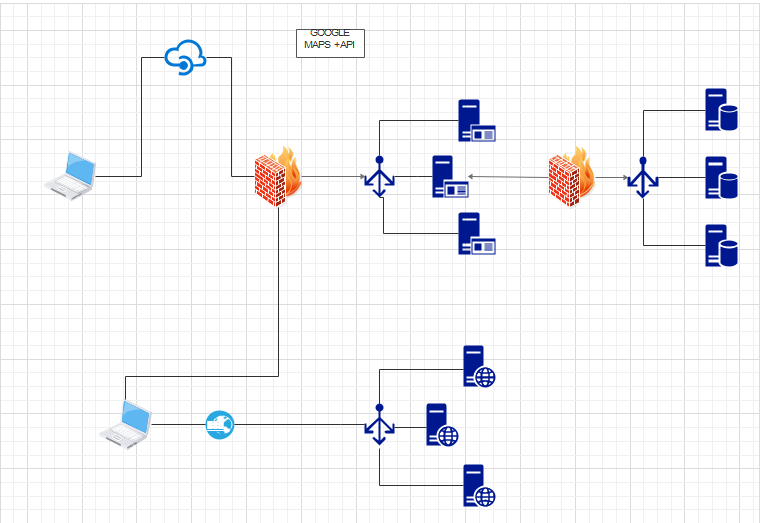
\includegraphics[width=0.98\linewidth, height=0.55\textheight]{Images/networkarchitecture}
	\caption{Network Architecture}
	\label{fig:networkarchitecture}
\end{figure}

The network architecture illustrates how the three-tier is applied to SafeStreets. The presentation level is all information that are shown on the web-app UI.

The authority own systems, that are not incorporated in the SafeStreets system, represent the software used to generate traffic tickets. They receive the data (type of violation, license plate, name, surname etc.) from the API that SafeStreets provides.

The application tier contains the web server and the application server. The web server provides the HTML pages and the JavaScript logic, to the web clients. 

The web server does not communicate with the application server because the contents of the web pages will be filled dynamically with the JavaScript calls between the authority/user device and the application server. 

With JavaScript asynchronous calls the client make and API call to some specific endpoints, by making a \textit{promise}.

The promise is resolved when the client receives data, in our case in JSON format, or the server communicate the HTTP status of the request made.
Contents of the pages can be updated when the JSON object is received.

The data access level contains the database server, that communicates with the application server.
The latter will interrogate the database server to retrieve, update or remove data.

The application server is connected with two firewalls.
They guarantee and improve security of the network and provide more controls on the packets that are sent through the network.

In order to grant better performances, every server is connected to a load balancer to distribute the request avoiding slowdowns.

The end devices exploit the browser cache to grant less requests.

\subsubsection{Database structure}
The database will have a structure according to the following one: 

\begin{figure}[H]
	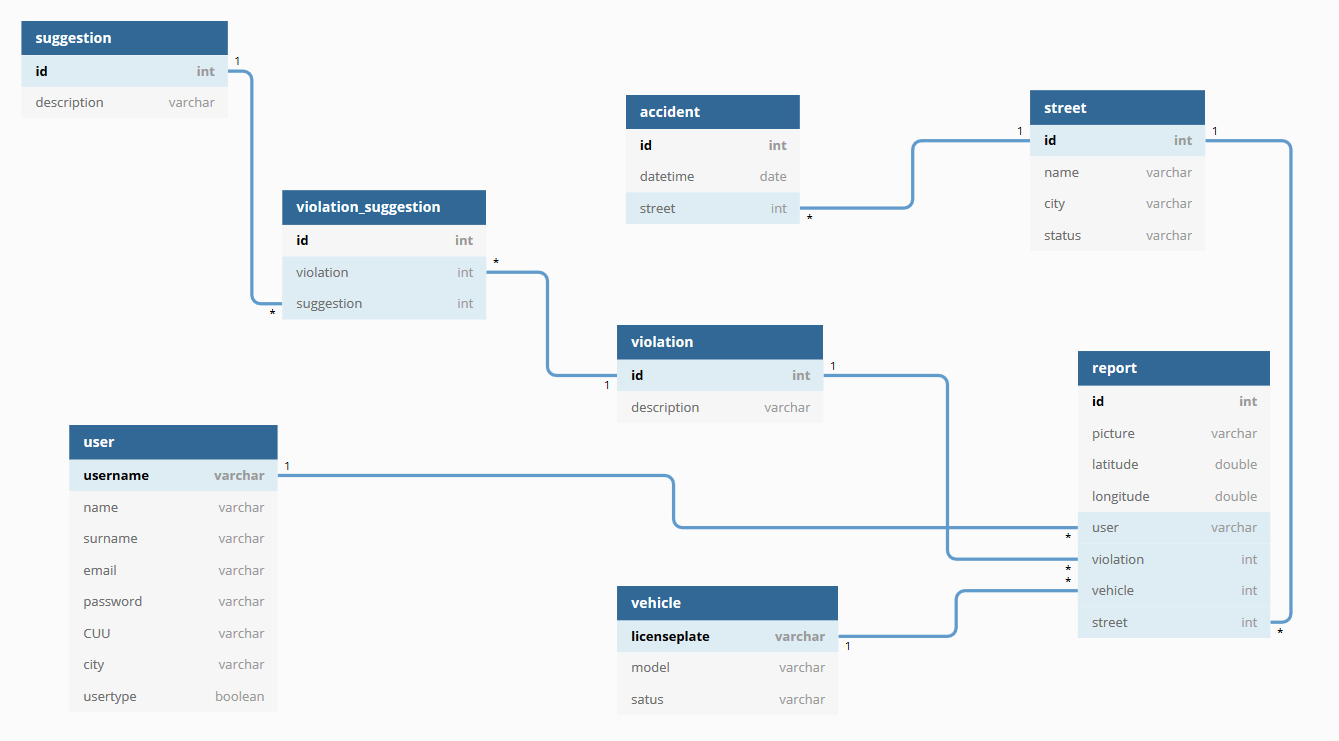
\includegraphics[width=0.95\linewidth, height=0.50\textheight]{../DD/Images/ER}
	\caption{Database structure}
	\label{Database structure}
\end{figure}


\subsection{Component view}
In order to give a better description of the component of the system, the class diagram below shows how the application is designed.

All this description regards only the application tier of the system.

Communication between client and the application is made by an interface exposed (SystemMangerInterface).
 
The client, used by end users and authorities that want to see statistics, does not contain any portion of the logic of the system (except for the GPS tracking). 

Thus it is a thin client and no class diagram has been made for it.

In diagram notes, it is possible to see which design patterns has been implemented (facade and singleton).

The data are stored in the database, are accessible using the manager classes. Their function is to query the database and save the data retrieved in the appropriate objects (for every entity of the database a specific class has been designed).

All the request arriving from clients are managed by the application server. Then it calls the appropriate method of facade class SystemMananger using the interface SystemMangerInterface. This class uses the methods of other classes to respond to the request.

A SystemManager method, used for obtaining information about accidents occurred, is called periodically. It retrieves the information and then stores them in the database.

During the registration process of an authority the specific method calls a web service to check the authenticity of the CUU code.

Moreover, an interface is exposed to authorities systems. In this way they can call a method that provide the reports data and generate traffic tickets on them. 

Before sending any type of information the identity of the authority is checked using the appropriate method of UserManager class.

\begin{figure}[H]
	\centering
	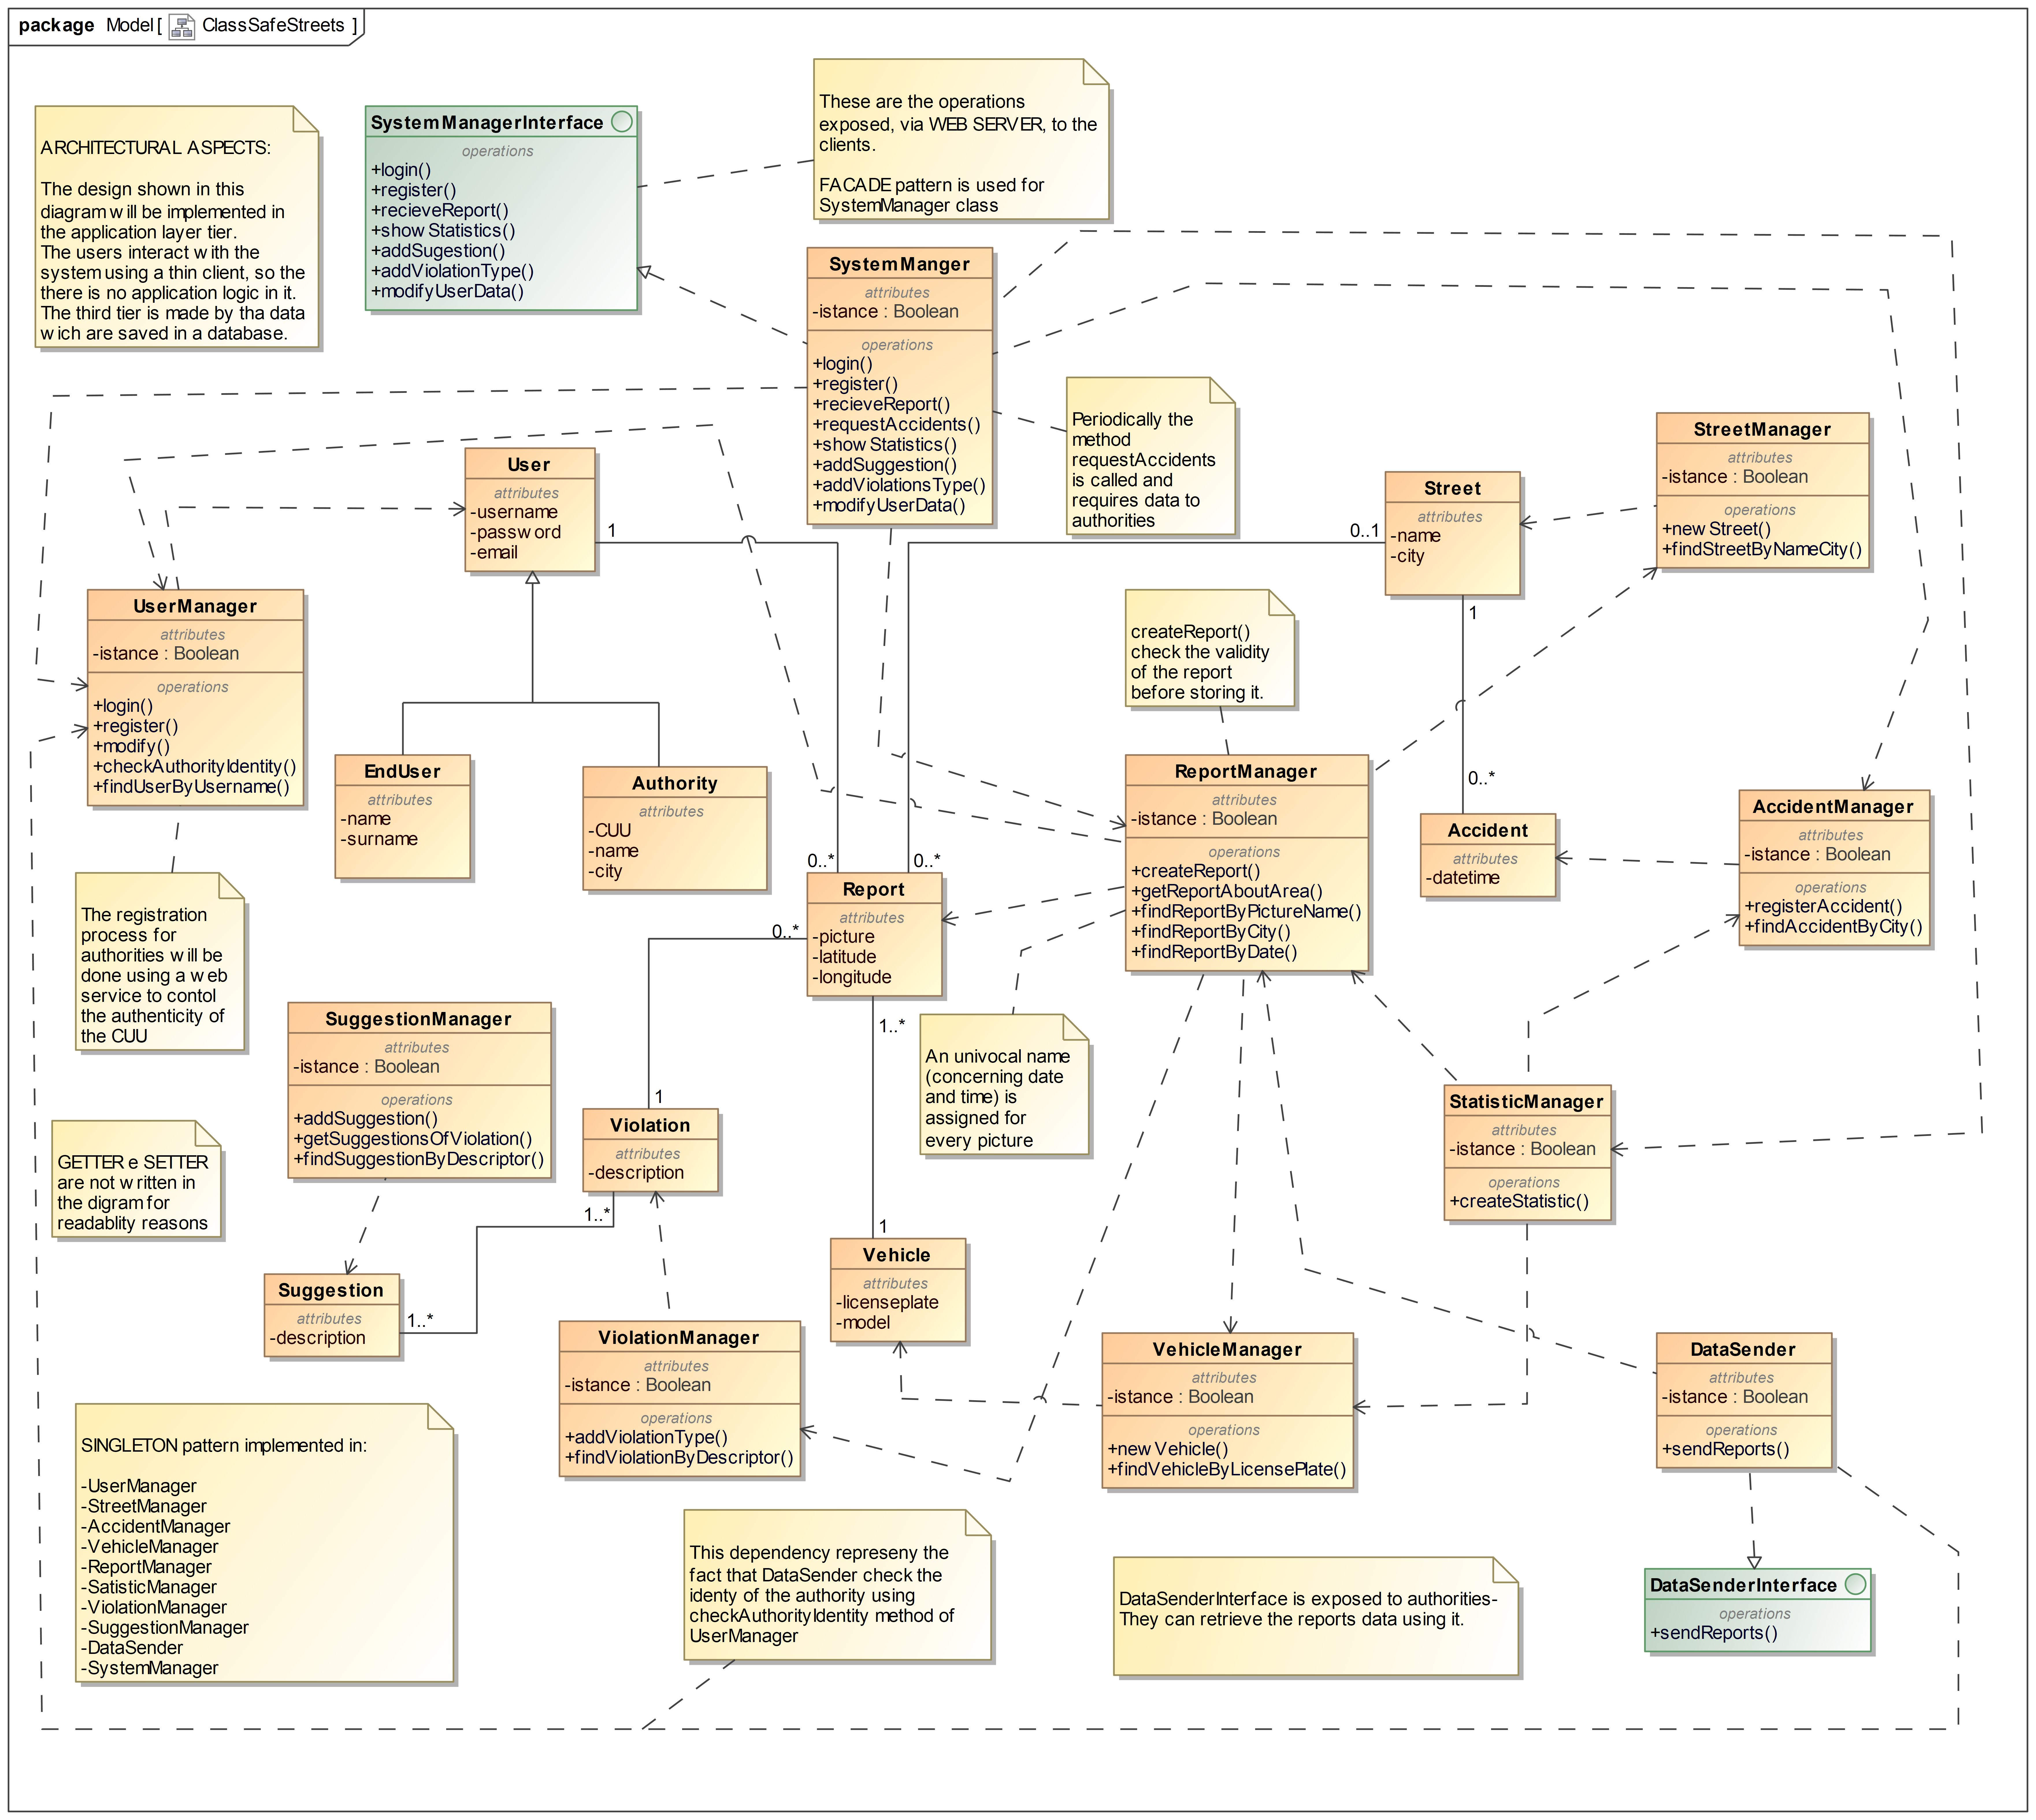
\includegraphics[width=1.12\linewidth]{Images/ClassSafeStreets.png}
	\caption{Class diagram}
\end{figure}

The component diagram below describes the implementation of the classes described before in terms of components.

The macro-component \textit{SafeStretsApplication} represents the Java application running on the application server. It exposes two interfaces: the first one is designed to communicate with the client. The second is exposed to authority systems in order to offer information that can be used to generate traffic tickets.

There are also sub-components that perform specific operations and interact with the database:
\begin{itemize}
 \item 
 SystemManager: is the component that conveys all the requests to appropriate sub-components and periodically activates the AccidentManager.
 \item 
 AccidentManager: is the component that calls the specific service to retrieve the data about accidents occurred. These information will be used by StatisticManager.
 \item
 StatisticManager: is the component designed to create statistic crossing data coming from report and accidents.
 \item 
 PositionManager: is the component used to organize data about position and streets.
 \item 
 UserManager: is the component used to manage user operations (for instance login,registration...).
 \item
 ReportSender: it is used to send data about reports stored to authority system. These information will be used to generate traffic tickets. This sub-component exposes directly an interface to the external environment. Naturally before sending the data, the method check the identity of the authority using the UserManager.
 \item 
 VehicleManager: is the component designed to manage the data about vehicle.
 \item 
 ViolationAndSuggestionManager: it is used to store and modify the type of violation and suggestion.
 \item 
 ReportManager: is the component that store reports in the database and retrieve information on it.
 \item 
 DatabaseManager: it is used to keep the connection to the DBMS and to send queries to it.
 
\end{itemize}

\begin{figure}[H]
	\centering
	\includegraphics[width=1.12\linewidth]{Images/component.png}
	\caption{Component diagram}
\end{figure}

\subsection{Deployment view}
In the deployment diagram below it is possible to see the physical implementation of the system.
SafeStreets is composed by 3 nodes:
\begin{itemize}
	\item 
	First tier: represent the thin client that make HTTP requests. It is used by users for sending reports and by authorities in order to see statistics.
	\item 
	Second tier: is made by the web server and the application server. The first one is responsible of the catching of the HTTP requests coming from the clients. The web server read the requests and call the appropriate method exposed by the application server. The real computation of the requests is done here.
	When data stored are required, the application server communicates with the third tier.
	\item 
	Second tier: this tier represents the database of the system. 
\end{itemize} 

In the diagram there is also another node that corresponds with the authority system in charge of retrieving reports to generate traffic tickets. The application server exposes a interface that provides this function. 

\begin{figure}[H]
	\centering
	\includegraphics[width=1.12\linewidth]{Images/Deployment.png}
	\caption{Deployment diagram}
\end{figure}

\subsection{Runtime view}
\newpage

\subsubsection{Registration}
The sequence diagram below shows how it is developed the registration of a new user. The SystemManager class , through its interface, calls  the method "register()" of the UserManager, giving three parameters: username, mail, password. The first two parameters must be unique otherwise the registration failed.
UserManager will call the method "insert()" of DatabaseManager that will recieve as parameter the User and will add it into the database.
\begin{figure}[H]
	\centering
	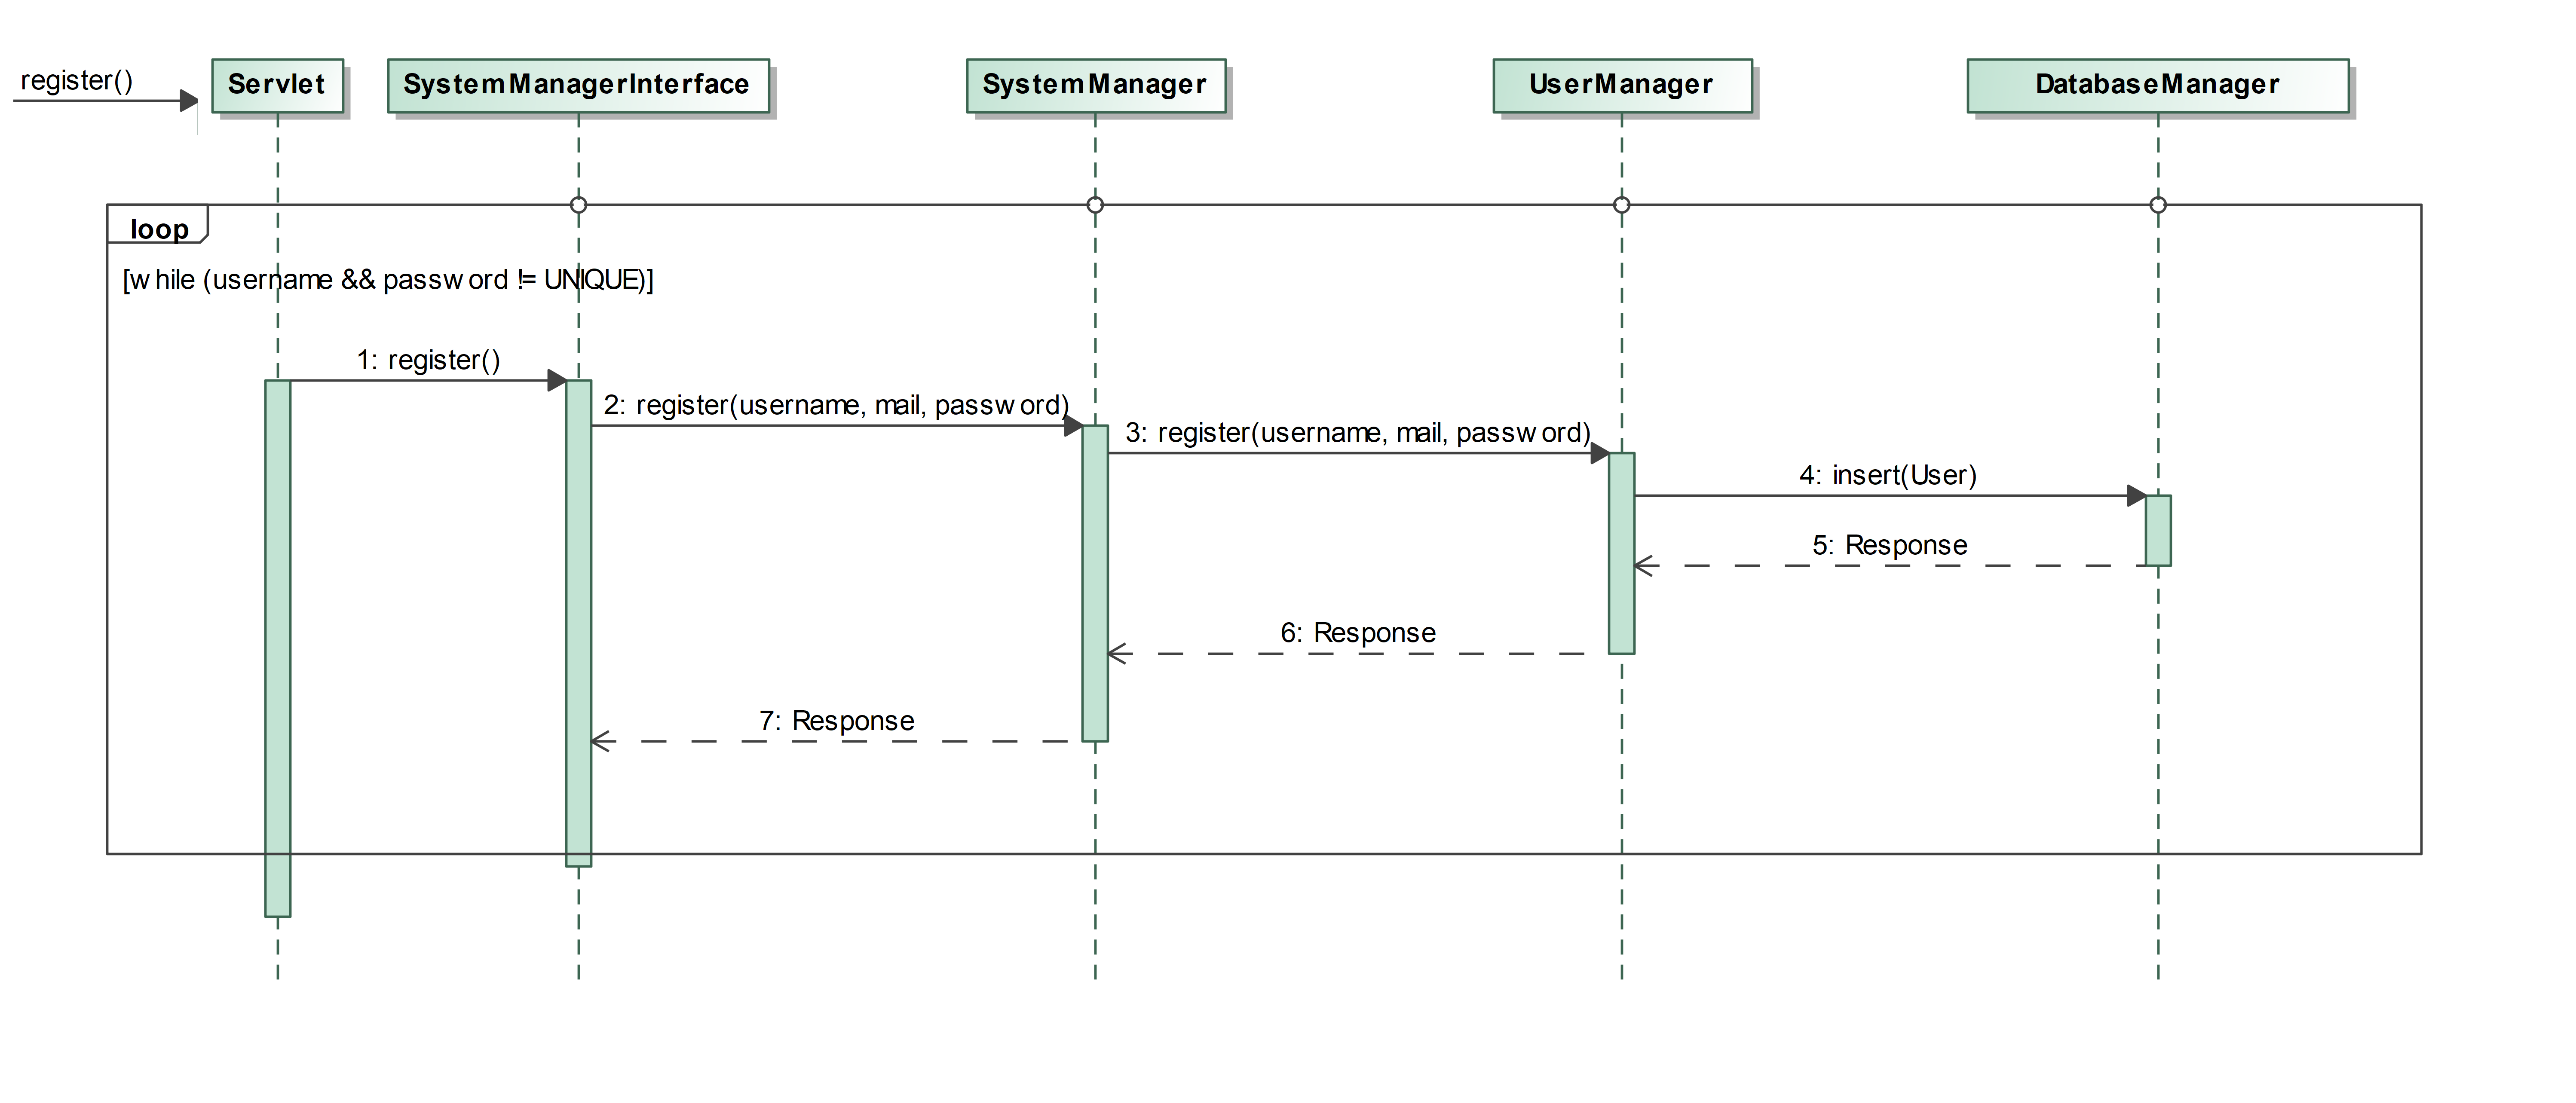
\includegraphics[width=0.97\linewidth, height=0.32\textheight]{Images/RunTimeDiagram/Sequence1}
	\caption{Register}
	\label{fig:Register}
\end{figure}
\subsubsection{User reports a violation}
The user log in using the method login through UserManager, SystemManager, SystemManagerInterface and DatabaseManager, giving username and password as parameters.
Than the SystemManager call the method recieveReport() that will place it in listen for the new report. The report is created and stored only if it is valid and consistent. The ReportManager will call createReport() that implies the communication with with DataSender and  DataSenderInterface using "sendReport()".
Once the report is recieved, if it is possible and aren't already present in the db, the street, the vehicle and the type of violation will be added in the db, through DatabaseManager, using the different manager: StreetManager, VehicleManager, ViolationManager with reciprocally the methods: newStreet(), newVehicle() and addViolationType().
\begin{figure}[H] 
	\centering
	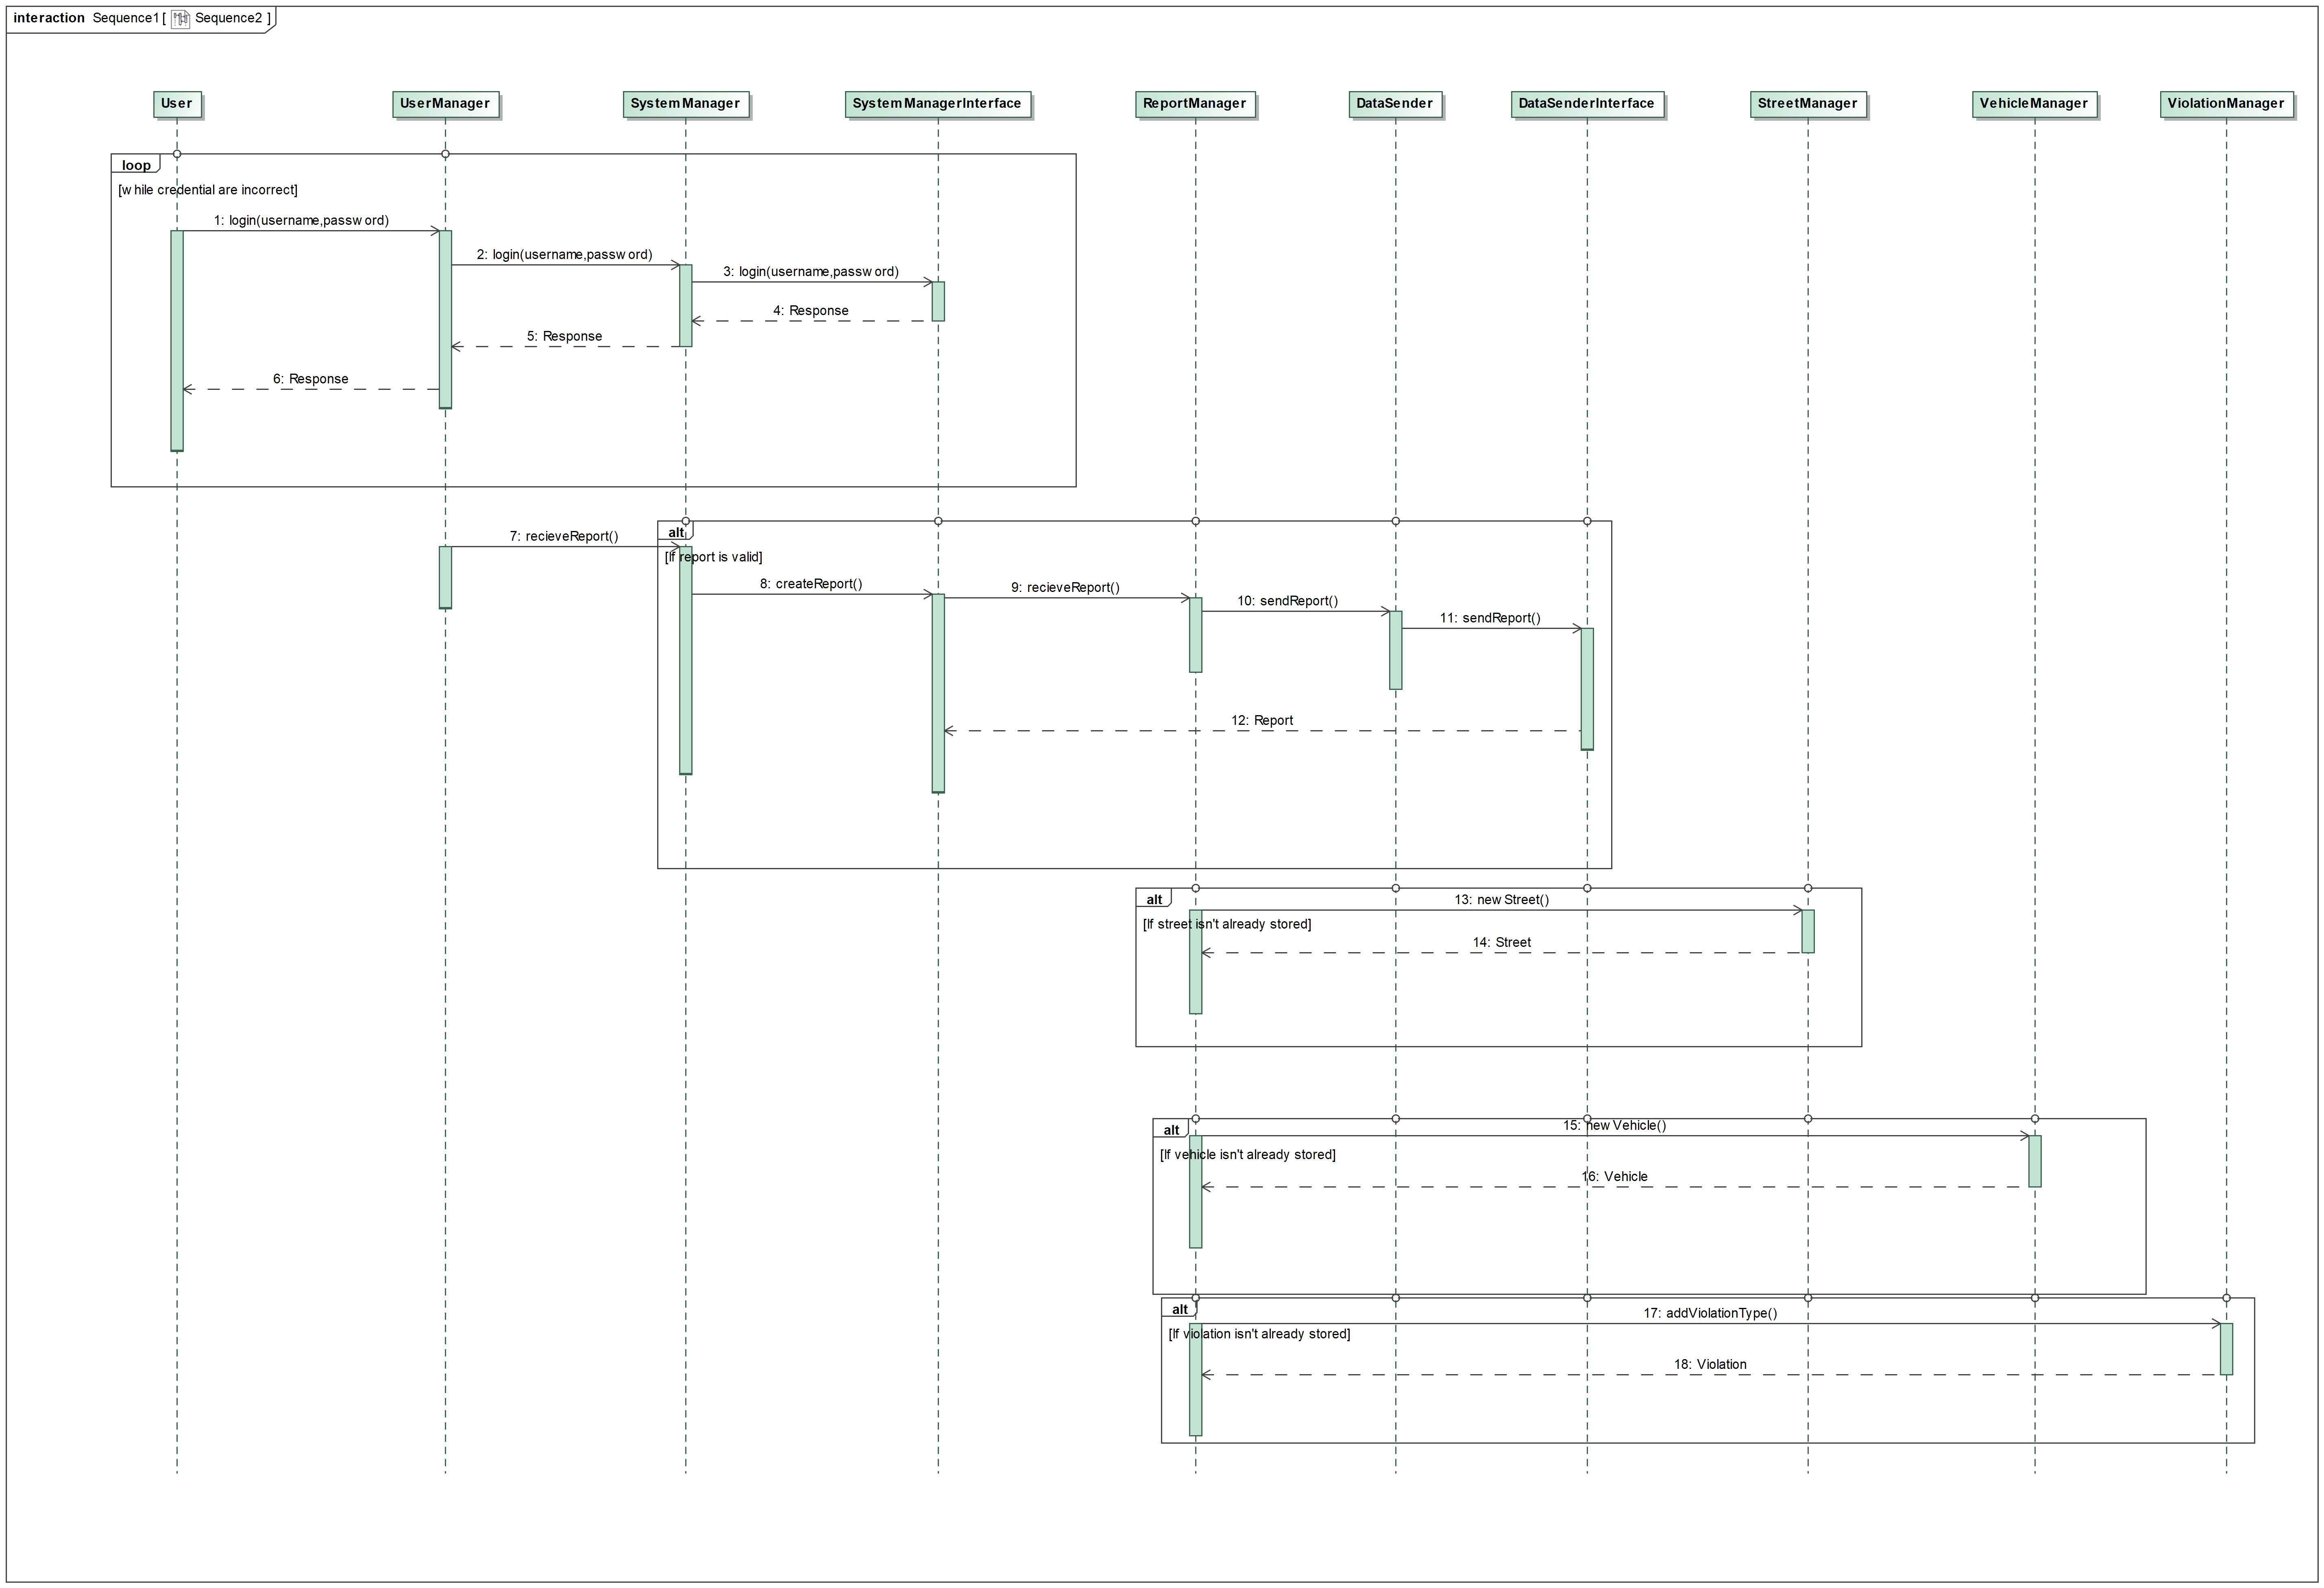
\includegraphics[width=0.95\linewidth, height=0.7\textheight]{Images/RunTimeDiagram/Sequence2}
	\caption{User reports a violation}
	\label{fig:User reports a violation}
\end{figure}
\subsubsection{Check report status}
The user after having logged in, the UserManager call findReportByUser() passing it the username and the ReportManager will retrieve the report. Using the getter and setter it is possible to see the report status.
\begin{figure}[H]
	\centering
	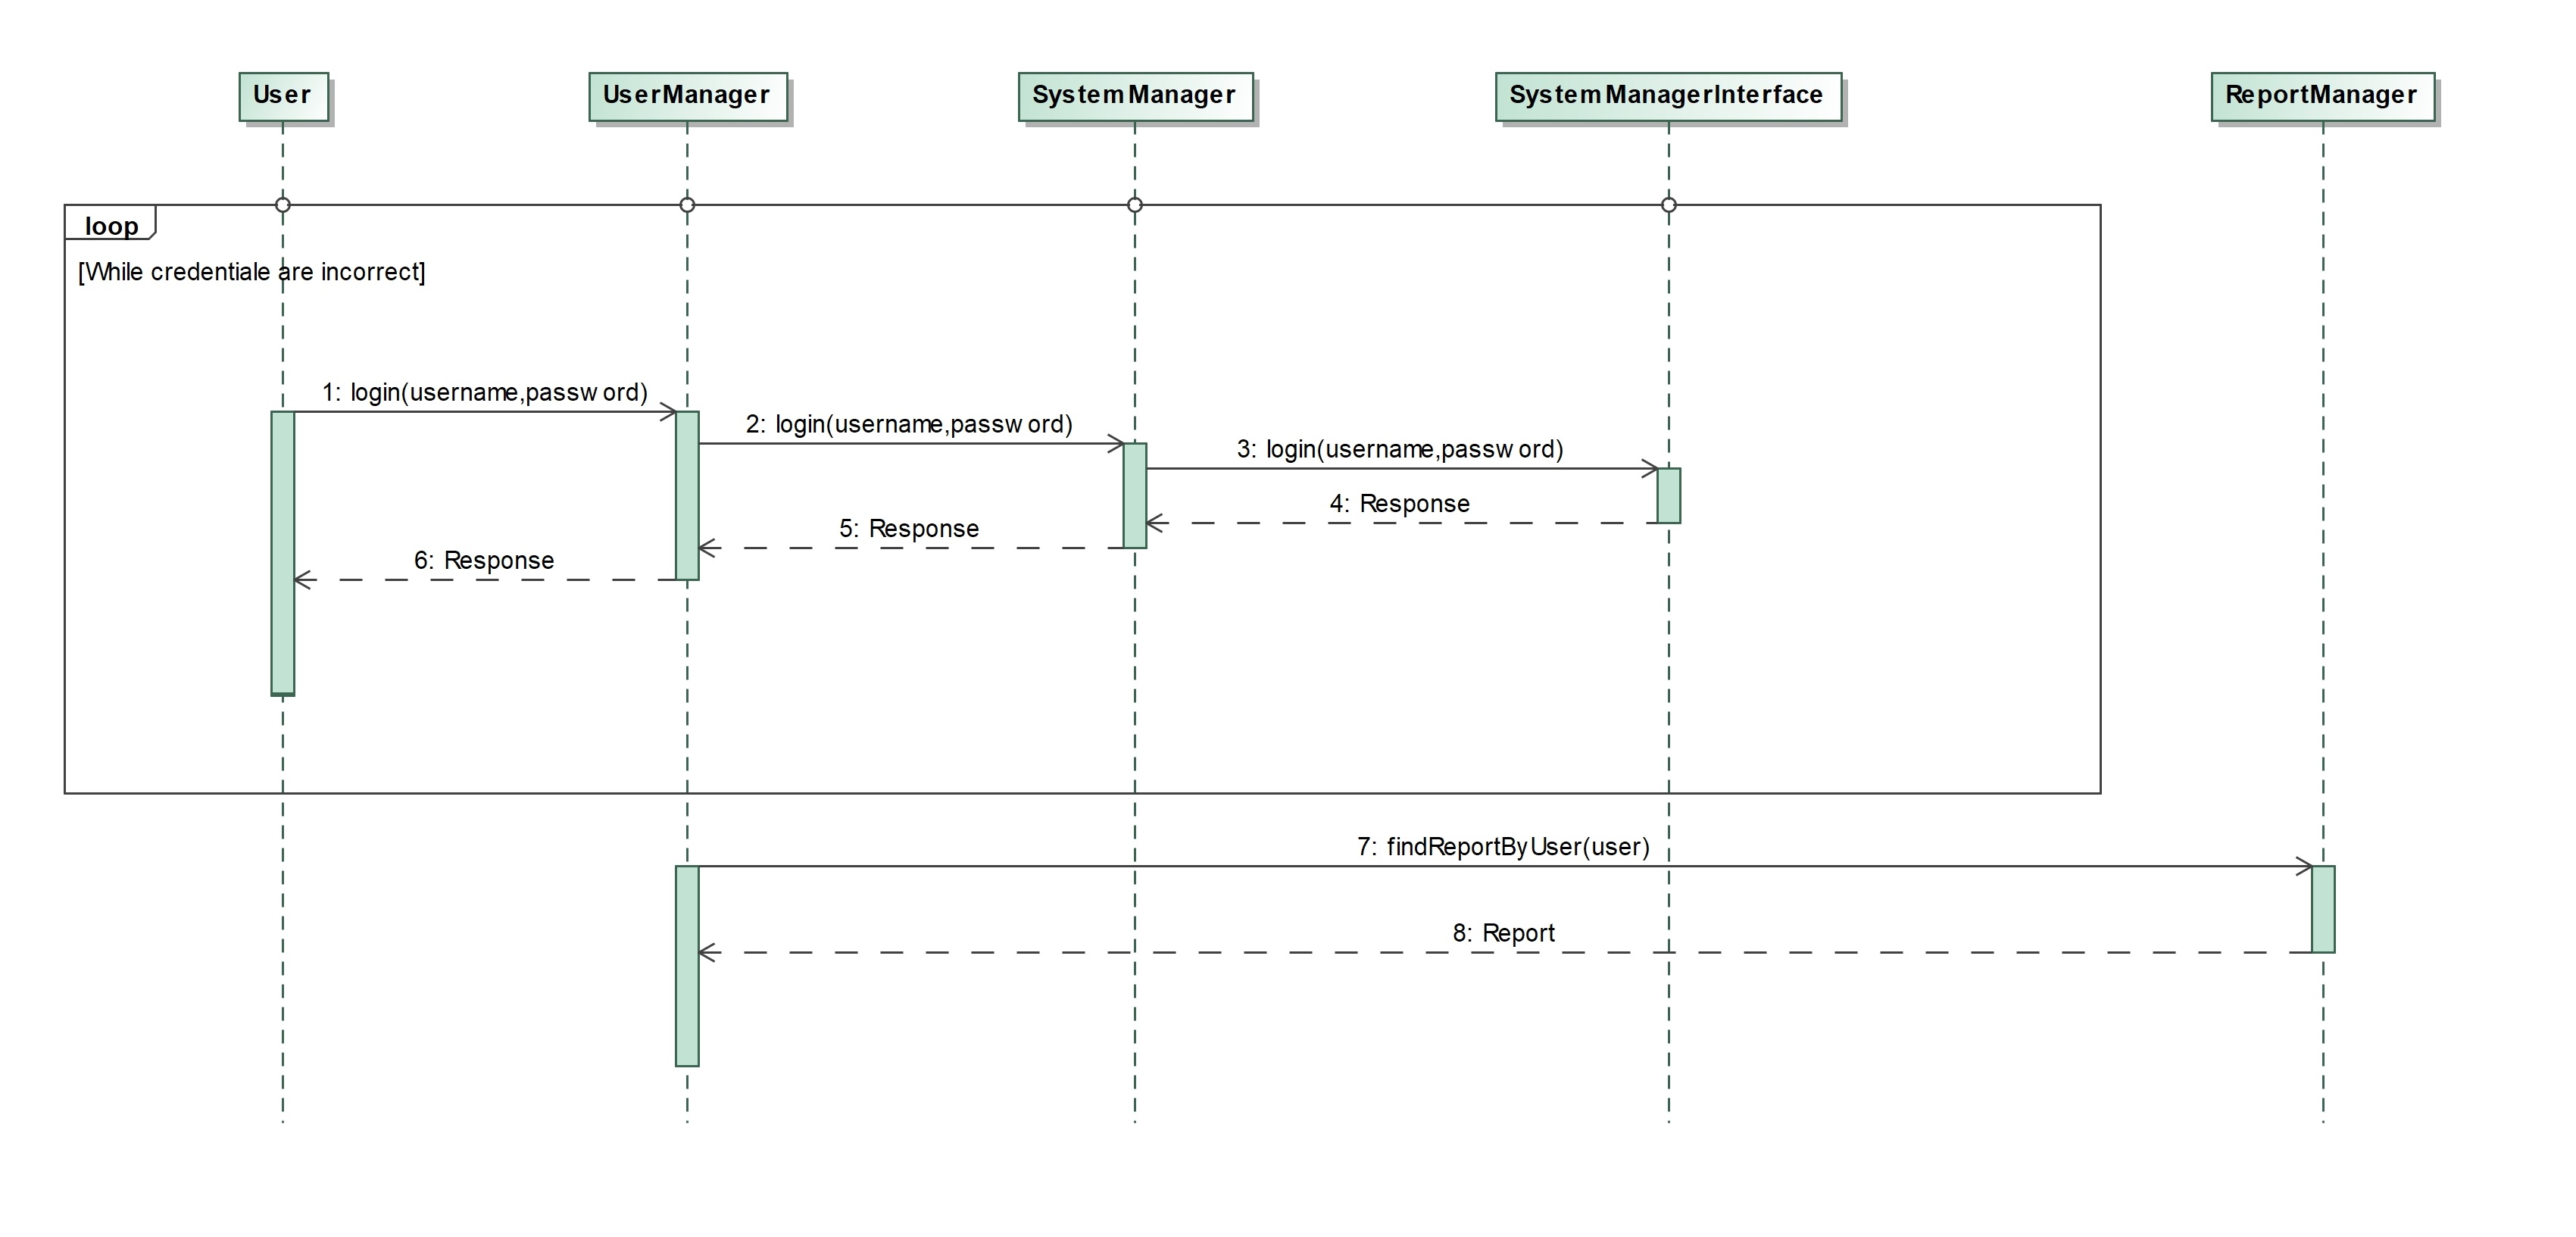
\includegraphics[width=0.95\linewidth, height=0.4\textheight]{Images/RunTimeDiagram/Sequence3}
	\caption{Check report status}
	\label{fig:Check report status}
\end{figure}
\subsubsection{Insert accident and generate statistic}
The Authority logs into the platform in a similar way as the user but instead giving his username, he will provide his CUU. Than from the SystemManager it will call registerAccident() on the AccidentManager(). The AccidentManager will call createStatistic() on the StatisticManager that will provide the statistic to the SystemManager, which call showStatistic() to display them.
The accident will be inserted into the database using the method "insert()" of DatabaseManager.
\begin{figure}[H]
	\centering
	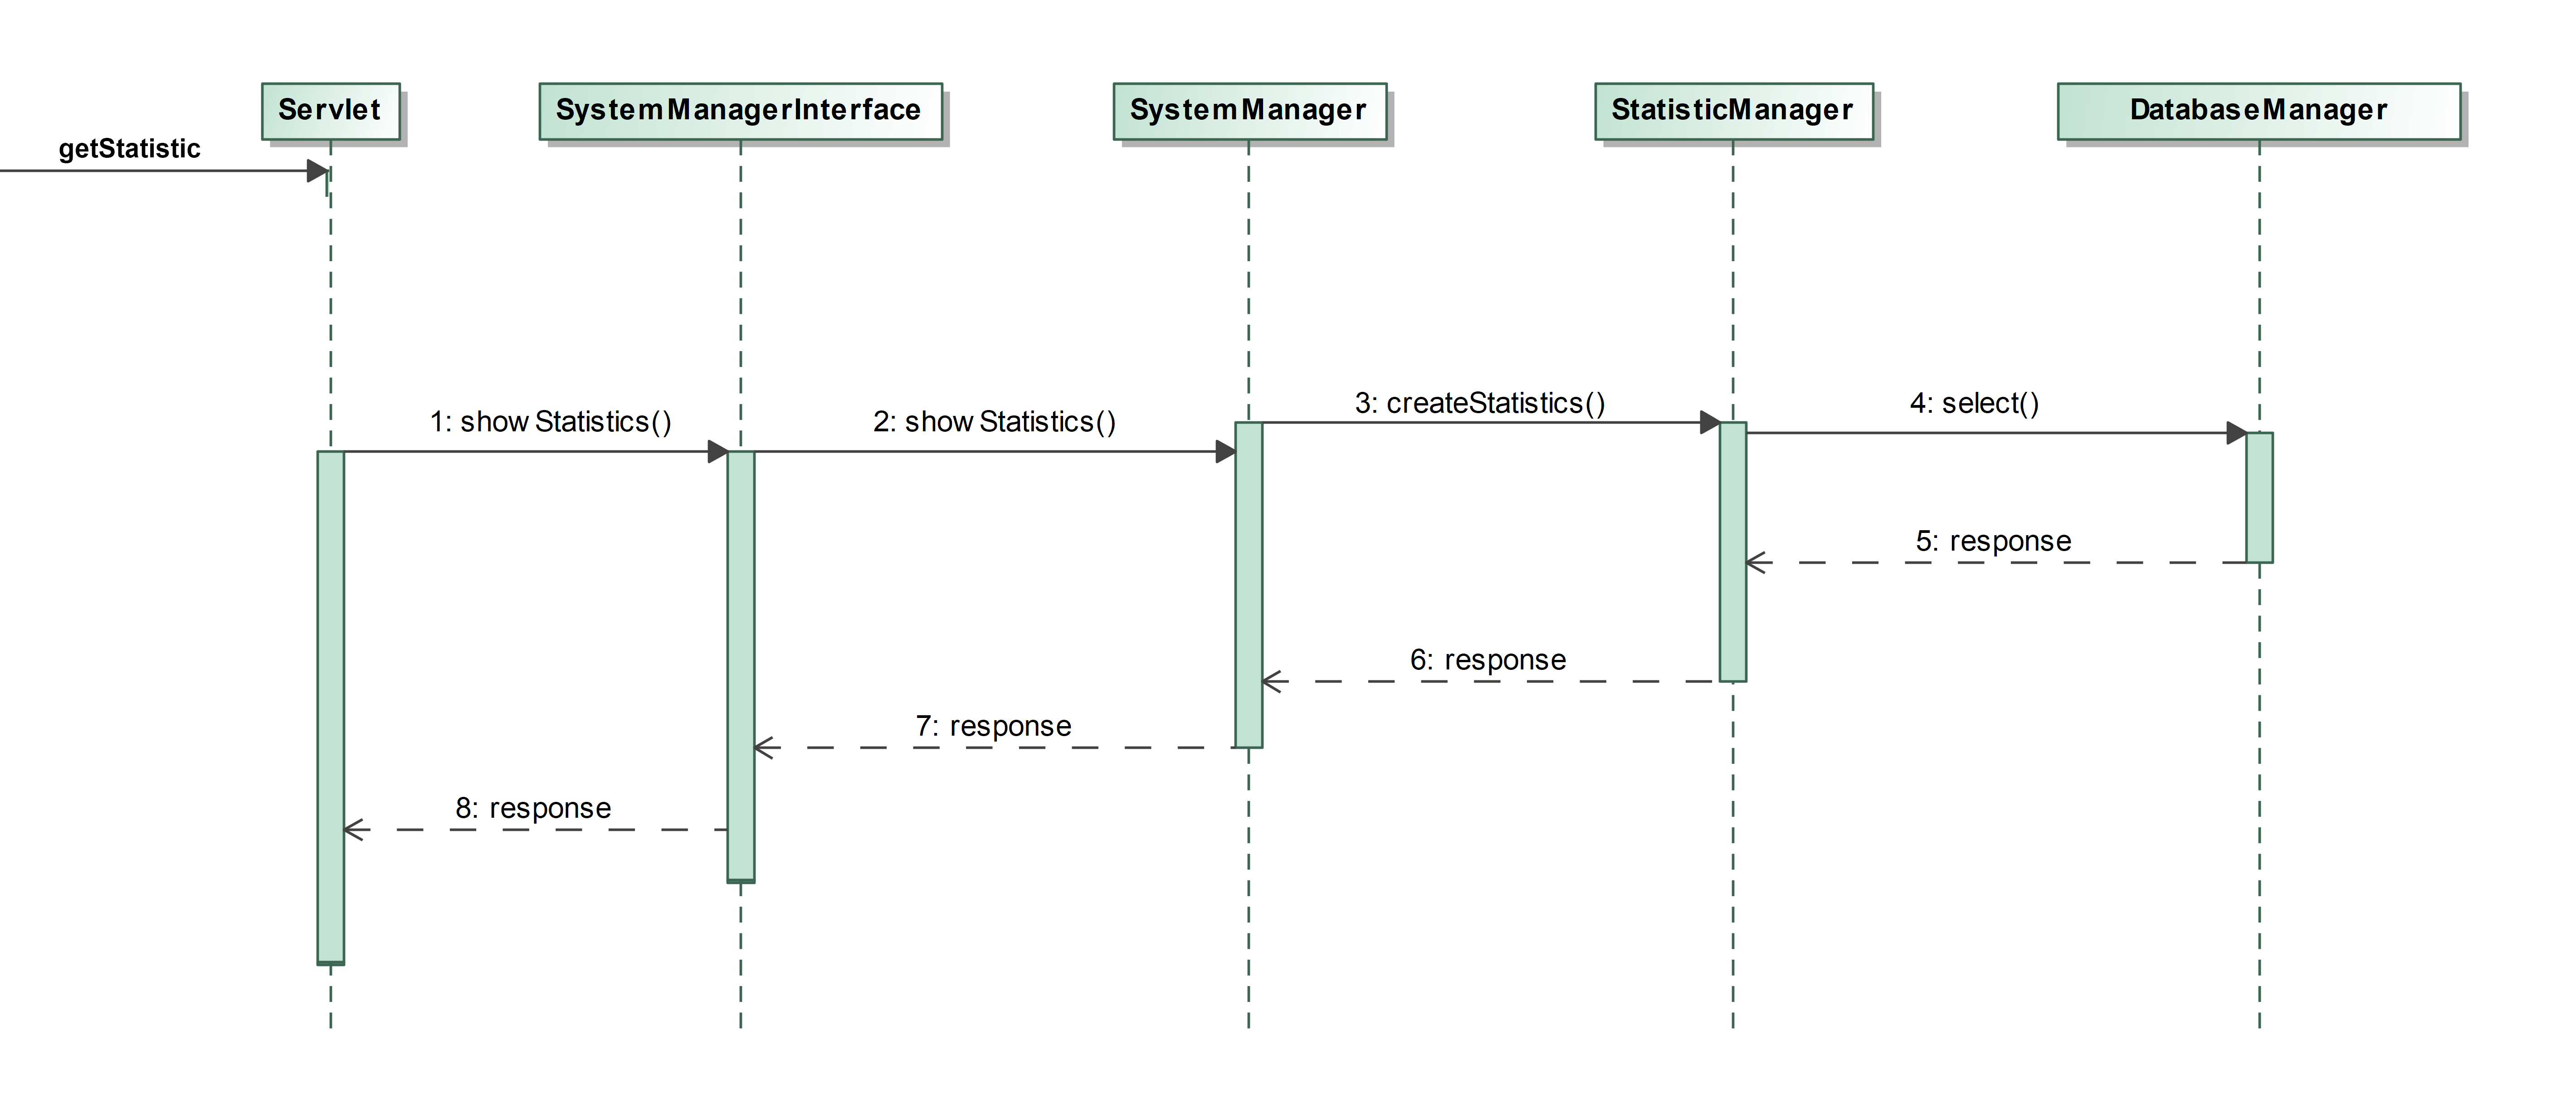
\includegraphics[width=0.95\linewidth, height=0.45\textheight]{Images/RunTimeDiagram/Sequence4}
	\caption{Insert accident and generate statistic}
	\label{fig:Insert accident and generate statistic}
\end{figure}
\subsubsection{Check street status}
The Authority after logging into the platform, will call findStreetByNameCity() from SystemManager to the StreetManager passing the city name as parameters. The StreetManager will give as response the Street, so it is possible to retrieve the street status using getter method.
\begin{figure}[H]
	\centering
	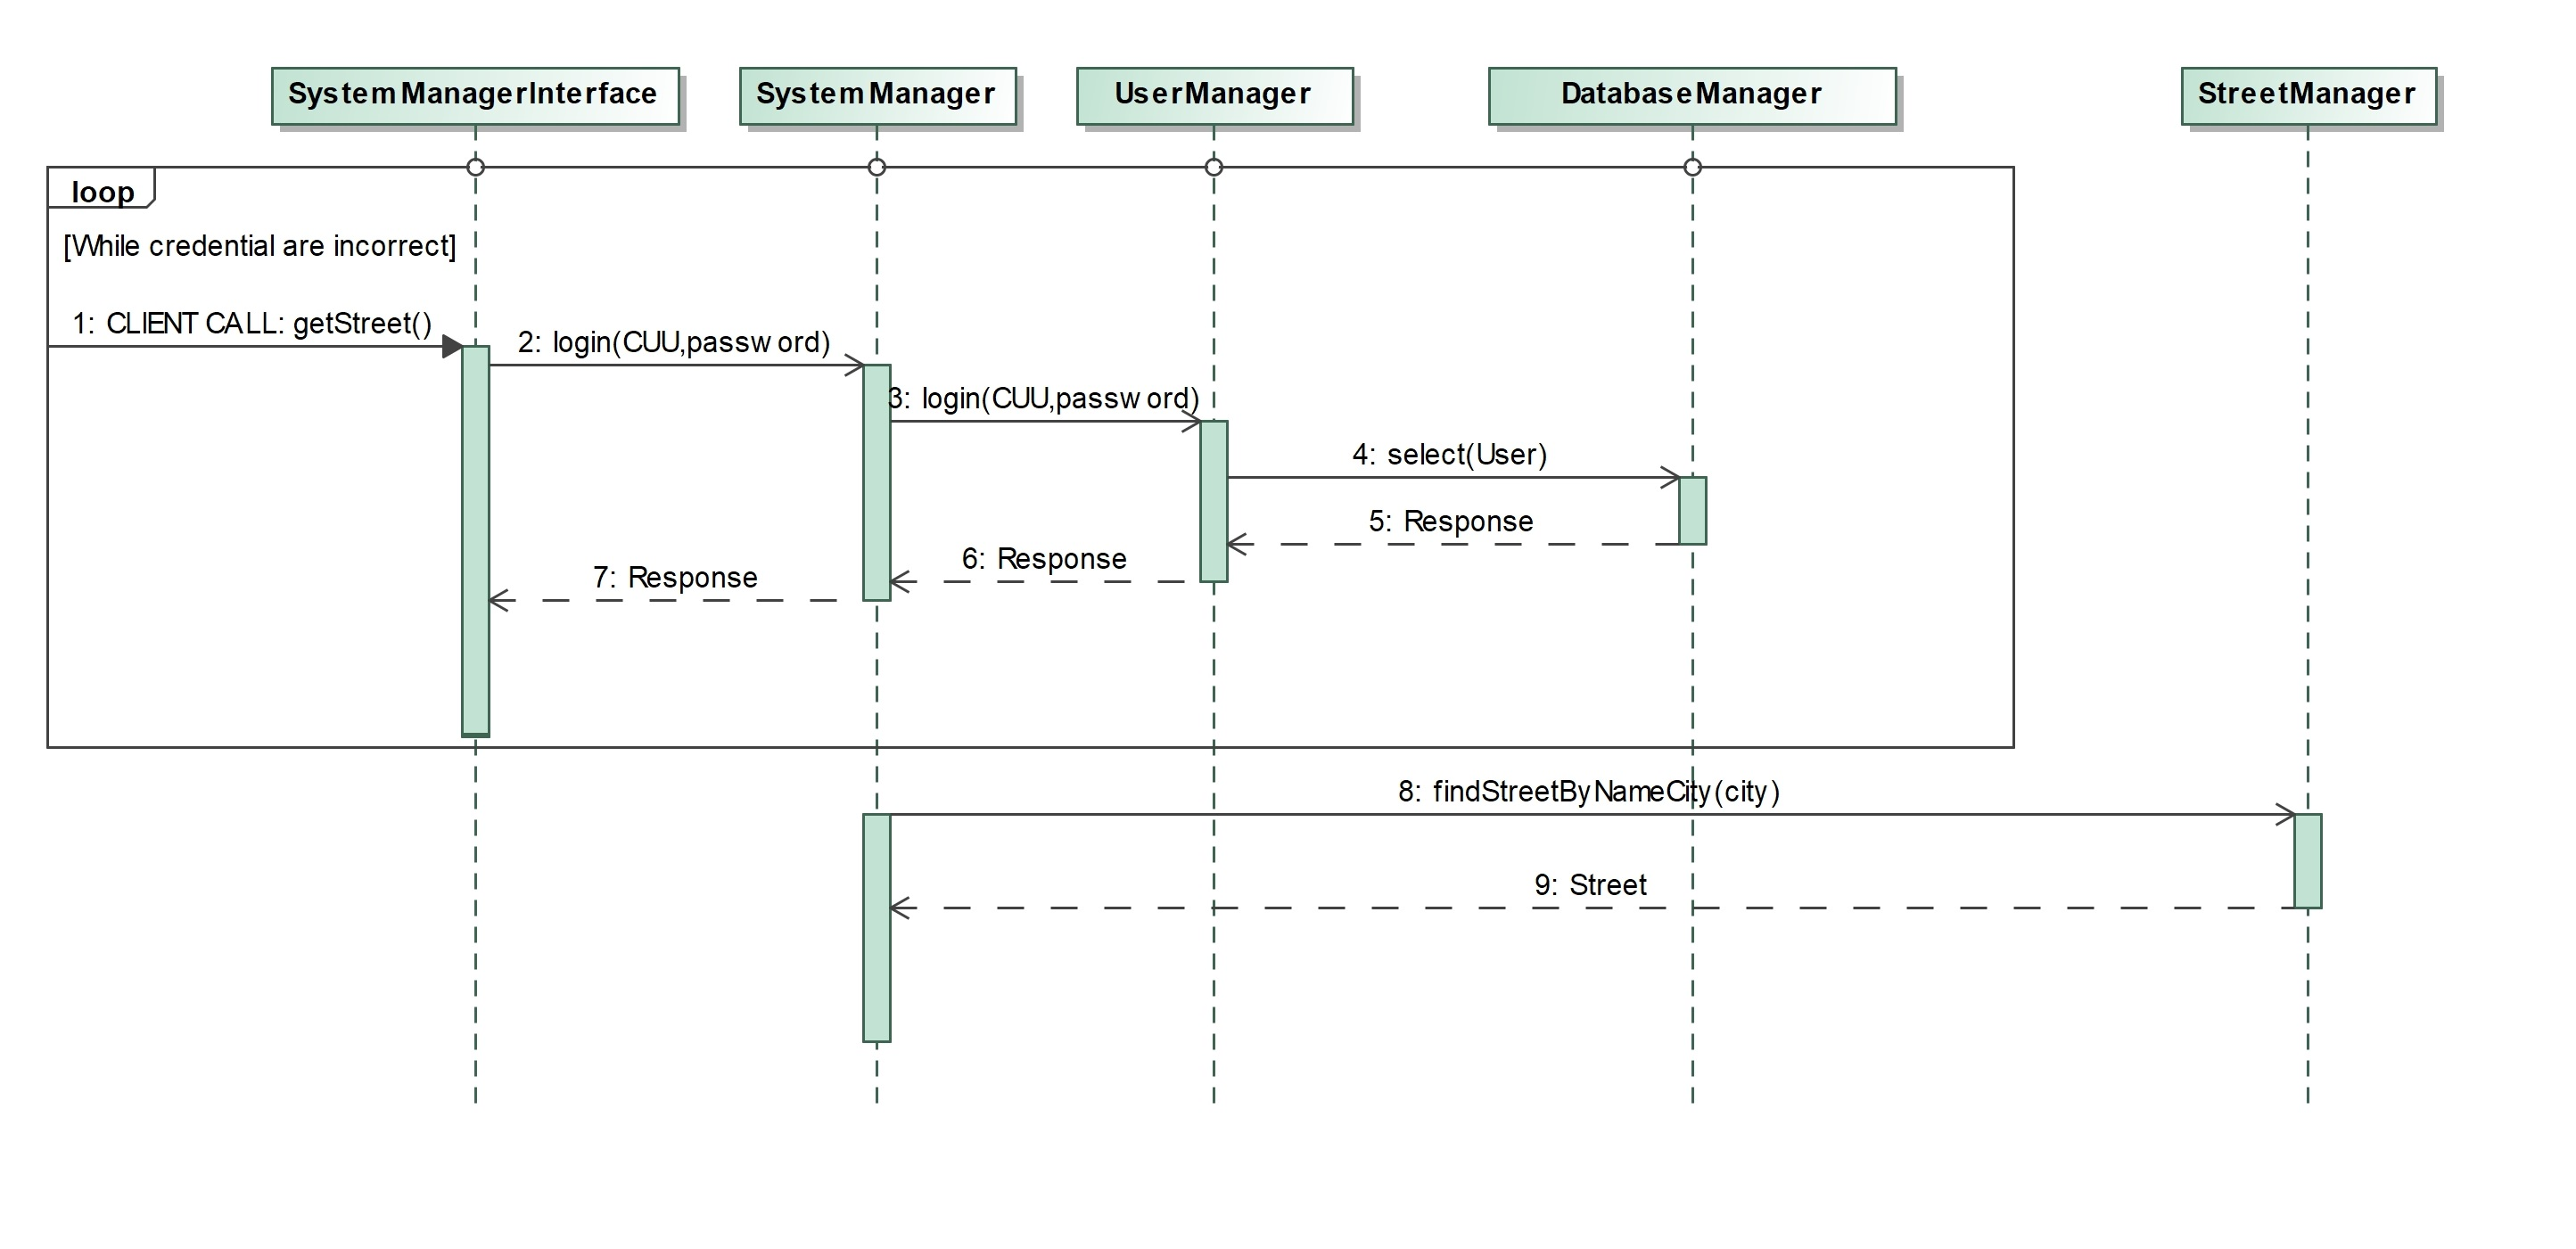
\includegraphics[width=0.95\linewidth, height=0.35\textheight]{Images/RunTimeDiagram/Sequence5}
	\caption{Check street status}
	\label{fig:Check street status}
\end{figure}
\subsubsection{Check car status}
The Authority after logging into the platform, will call findVehicleByLicensePlate() from SystemManager to the VehicleManager passing the license plate as parameters. The StreetManager will give as response the Car, so it is possible to retrieve the car status using getter method.
\begin{figure}[H]
	\centering
	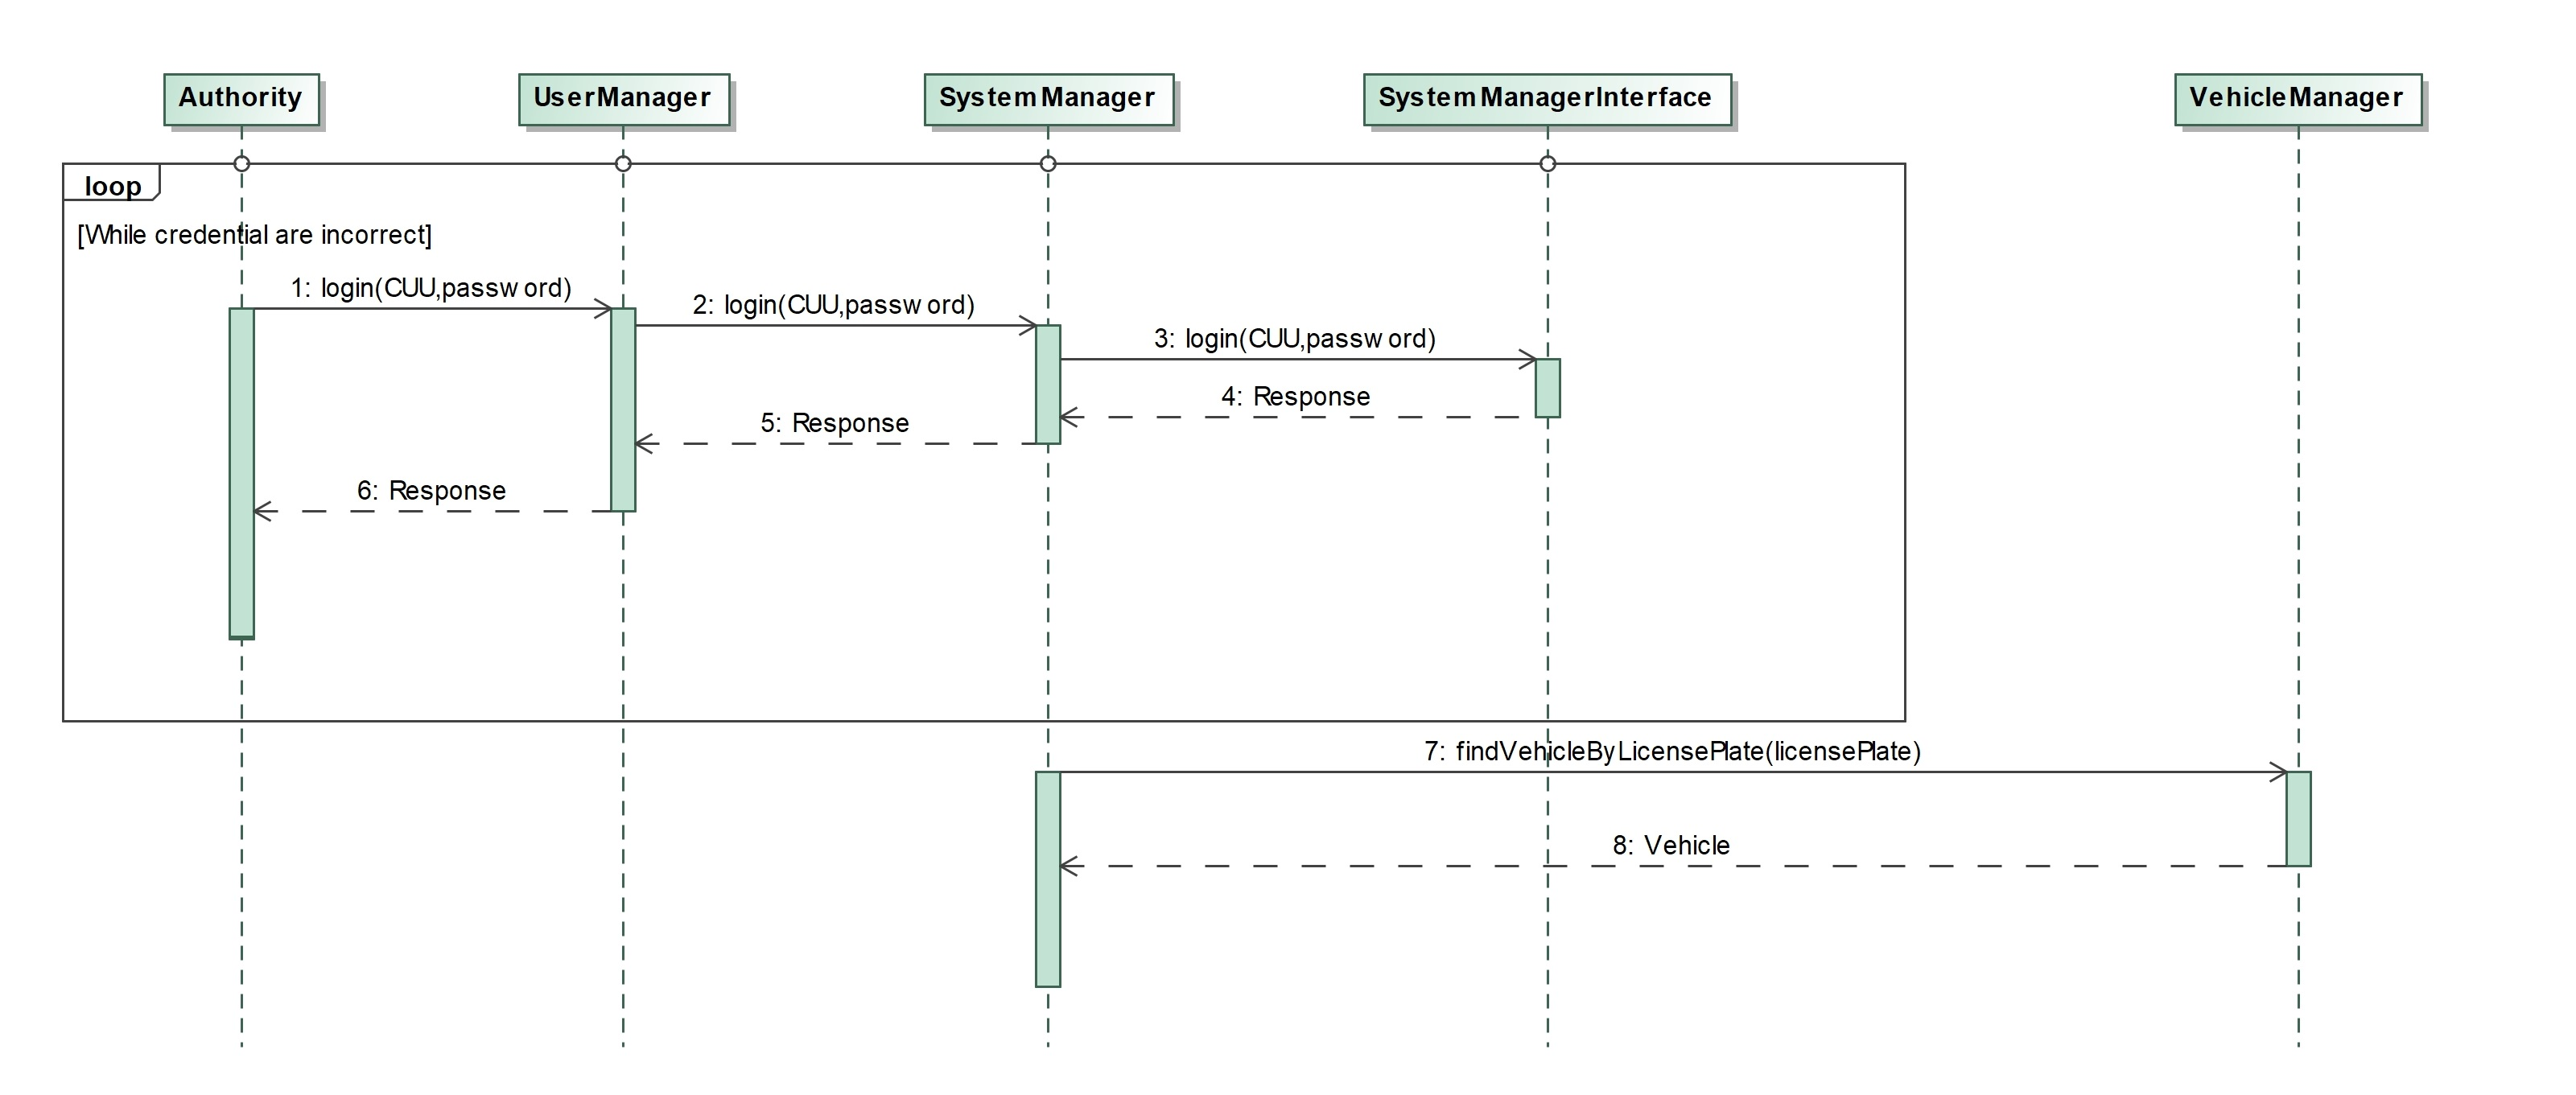
\includegraphics[width=0.95\linewidth, height=0.35\textheight]{Images/RunTimeDiagram/Sequence6}
	\caption{Check car status}
	\label{fig:Check car status}
\end{figure}


\subsection{Component interfaces}

The interfaces exposed are manly two: SystemManagerInterface and DataSenderInterface. Their role was explained in the previous sections of this document.

\begin{figure}[H]
	\centering
	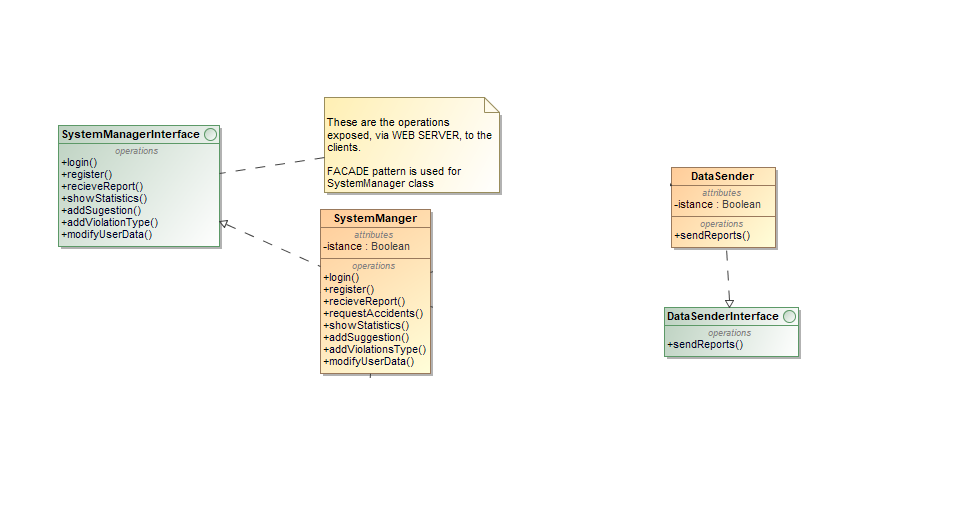
\includegraphics[width=1.12\linewidth]{Images/ComponentInterfaces.png}
	\caption{Component interfaces}
\end{figure}


Here the focus is on the feature provided by the methods exposed.

\subsubsection{SystemManagerInterface}
Every method exposed by this interface will correspond to a servlet that is able to catch the request and return data to the client.
\begin{itemize}
	\item 
	User login(String user, String password)
	
	It is the method in charge of checking the identity of the user/authority that want to log in the application. It returns the object User if the login process was successfully done, otherwise the object is null. 
	
	The application server checks the type of User object returned and then generates the proper response.
	The method works by invoking methods of UserManger class.
	
	\item 
	User register(String user, String password, String mail, String name, String surname)
	
	This method does the registration of a normal user and returns the User object as login method. Since the username has to be univocal the process can abort, in this case a null object is returned.
	Reading the returned object, the application server will generate the proper response.
	The method works by invoking methods of UserManger class.
	
	\item 
	User register(String user, String password, String mail, String name, String CUU, String city)
	
	This method does the registration of an authority user and returns the User object as login method. Since the username has to be univocal and the CUU is checked here (via Web Service), the process can abort, in this case a null object is returned.
	Reading the returned object, the application server will generate the proper response.
	The method works by invoking methods of UserManger class.
	
	\item
	 Bool recieveReport(String picture, Double latitute, Double longitude, String Violation, String violation, String licenseplate, String user, String city, String streetName)
	 
	 This method creates the report. During this process all the checks concerning the authenticity of the picture are performed and the coordinates are transformed into street name and city. In case the operations ends successfully, the proper objects (Report, Vehicle, Street) are created or associated (Violation, User) and then all data will be stored in the database. The picture name will be renamed with an univocal key made on date, time and user. A true value is returned.
	 In case of bad result on the checks of the authenticity, a false value will be returned.
	 According to the value returned by the method, the application server will generate the proper response. 
	 These operations will be performed using methods of ViolationManager, UserManager, ReportManager, VehicleManager and StreetManager.
	 
	 \item
	List<Integer> showStatistics (String user, String city)
	
	This method before generating statistics regarding the city, checks the identity of the user. 
	If the username does not correspond to an authority, it returns a null value.
	Otherwise it generates statistics using data of reports and accidents referred to the city.
	According to the result of the method the application server generates the proper response.
	This method works using UserManager and StatisticManager classes.
	
	\item 
	Bool addSuggestion (String user, String description)
	
	This method before adding the suggestion, checks the identity of the user. 
	If the username does not corresponds to an authority, it returns a false value.
	Otherwise it adds the suggestion into the list and returns true.
	According to result of the method the application server generate the proper response.
	This method works using UserManager and SuggestionManager classes.
	
	\item 
	Bool addViolationType(String user, String description)
	
	This method has the same behavior of the previous one regarding the suggestions.
	
	\item 
	Bool modifyUserData(String oldPassword, String email, String newPassword)
	
	The method updates the data if the username exists and the old password is correct, then
	a boolean value is returned. According to result of the method, the application server generate the proper response.
	The method use UserManager class to perfom that opertaion.
\end{itemize}

\subsubsection{SystemManagerInterface}

The only method of this interface is sendReports:
\hfill

List<Report> sendReport (String username, String password, String city, Date date)



The method checks the user's identity using username and password. If it results a profile of an authority, a list of report done in the city on that date is provided to the caller. Otherwise a null value is returned.
The process works using ReportManager class and without involving the web server.


\subsection{Selected architectural styles and patterns}

\subsubsection{RESTful architecture}
SafeStreets adopts RESTful architecture. The main advantage of this architecture is the total separation between the user interface, from the server and the data storage.

RESTful is the architectural style of the web itself, for this reason developers with knowledge in web architecture will naturally develop in the RESTful architecture which is also simple and lightweight.

Client context is never stored on the server between requests, for this reason each request has to contain all the necessary information. 
A stateless server improves scalability because it allows the server to quickly free resources.

Using a RESTful architecture implies the adoption of the constraints illustrated below.
By operating within these constraints, the system gains desirable non-functional properties

\paragraph{Stateless}
It means that the necessary state to handle the request is contained within the request itself and server would not store anything related to the session. In REST, the client must include all information for the server to fulfill the request whether as a part of query params, headers or URI.

\paragraph{Uniform interface}
This constraint is fundamental to the design of any RESTful system and it is divided into:
resource identification in requests and individual resources are identified in requests (e.g. using URIs in RESTful Web services). 

\paragraph{Cacheable}
Caching, that can be implemented on the server or client side, shall be applied to resources when applicable and these resources have to declare themselves cacheable.

Caching partially or completely eliminates some client–server interactions, further improving availability and performance.

\paragraph{Layered system}
An application architecture needs to be composed of multiple layers. Each layer does not know anything about any layer except for the immediate one. 

Intermediary servers may improve system availability by enabling load-balancing and by providing shared caches.

\paragraph{Code on demand}
It is an optional feature. According to this, servers can provide executable code to the client.

\paragraph{Client–Server}
REST application must have a client-server architecture. Client does not need to know anything about business logic and server does not need to know anything about front-end, so they can change independently.


\subsubsection{Client-Server architecture}
Client–server model is an application structure that separates tasks between the providers of resources or services called servers, and multiple entities that request resources or services called clients.

In our case, client is the web-app from which users and authorities can access to SafeStreets through the browser, both mobile and desktop.

As described above, Client-Server architecture is a constraint that defines a RESTful system.

\subsubsection{MVC pattern}
This pattern is used to separate application concerns.
\begin{itemize}
	\item \textbf{Model}: It is the application data structure and directly manages the data, logic and rules of the application.
	\item \textbf{View}: View represents the visualization of the data that model represents.
	\item \textbf{Controller}: It communicates data back and forth between the Model objects and the View objects.
\end{itemize}

Because MVC divides the various components of an application, developers are able to work in parallel on different components without blocking others. 

SafeSteets is divided between the front-end and the back-end. Back-end developers design the structure of the data and how the user interacts with it without requiring the UI. Instead, front-end developers are able to design the UI of the web-app prior to the data structure being available.
Cons: Knowledge on multiple technologies becomes the norm. Developers using MVC need to be skilled in multiple technologies.


\subsubsection{Facade pattern}
Facade pattern is used in SafeStreets class diagram: \textit{SystemManagerInterface} and \textit{DataSenderInterface}.

It is used to cover the complexities of a large system and therefore provides a simple interface to the client. 


\subsubsection{Singleton pattern}
Singleton pattern is used in SafeStreets class diagram: \textit{UserManager, StreetManager, AccidentManager, VehicleManager, ReportManager, StatisticManager, ViolationManager, SuggestionManager, DataSender, SystemManager}.

By definition it is a pattern design that restricts the number of instances of a class to one object, so it is used when we need to have only one instance of our class.


\subsection{Other design decisions}

\subsubsection{Front-end}

\paragraph{React}

For the front-end, SafeStreets uses React JS, a modern JavaScript framework developed by Facebook.

React allows developers to create large web applications which can change data, without reloading the page. The main purpose of React is to be fast, scalable, and simple.

\textbf{JSX} is used for templating, instead of using regular JavaScript. It is simple JavaScript which allows HTML quoting and uses these HTML tag syntax to render components.

\subsubsection{Back-end}

\paragraph{Spring Boot}

For the back-end SafeStreet uses Spring Boot, is an application framework for the Java platform.
It is an already configurated Spring solution for creating stand-alone, Spring-based applications. It is an HTTP- and servlet-based framework for web applications and RESTful web services.

\subsubsection{Database}

\paragraph{MySQL}

SafeStreets uses MySQL as RDBMS (\textit{Relational DataBase Management System}) to store its data.
Structured relationships between rows and columns in a table, SQL databases are best when you need ACID compliance. 

ACID stands for:
\begin{itemize}
	\item Atomicity: each transaction either succeeds completely or is fully rolled back.
	\item Consistency: data written to a database must be valid according to all defined rules.
	\item Isolation:  when transactions are run concurrently, they do not contend with each other, and act as if they were being run sequentially.
	\item Durability: once a transaction has been committed to the database, it is considered permanent, even in the event of a system failure.
\end{itemize}






